\section{The TSTL Harness Language}

The TSTL compiler takes as input a harness template file, and produces
as output a Python class file that implements an interface other tools
can use to perform testing on the SUT, according to the harness details.

The harness in Figure \ref{fig:MakeFeatureLayer} shows many of the
basic features of TSTL.  The basic structure of a TSTL harness
consists of three parts, usually written in order.  First, harness
code prefixed by an {\tt @} or enclosed in {\tt <@ @>} is treated as
raw Python code, and essentially not interpreted by the TSTL
compiler.  This code is reproduced almost literally in the output
file\footnote{TSTL does have to scan {\tt import}s to properly
  implement restarting of testing, and also pre-processes function
  definitions to add a {\tt pre} construct to Python to support
pre- and post-conditions.}.  Second, there is a preamble that almost
always defines a set of \emph{value pools} for use in testing, but
also may include information on logging, correctness properties,
source code locations for code coverage analysis, and other basic
information that applies to the entire harness.  Finally, the bulk of
a TSTL harness (and the only absolutely required element) is a set of
\emph{actions}.  Actions are the possible steps to be taken in
testing, and define the set of possible tests.

The original version of TSTL \cite{NFM15} required cumbersome use of Python
functions to implement many simple operations.  Current TSTL extends
the language to make it possible to define complex test spaces
using only pools and actions.

\subsection{The Essentials of Pools and Actions}

In TSTL, tests consist of assignments to value pools and uses of the
values in those pools.  In order to make the core ideas clear,
consider a portion of Figure \ref{fig:MakeFeatureLayer} to
generates values for use in SQL where clauses:

{\scriptsize
\begin{code}
pools:
  <val> 2 CONST
\vspace{0.05in}
actions:
\vspace{0.05in}
<val> := <1..10>
<val> = <val> + 1
\end{code}
}

This, by itself, is a valid TSTL harness.  There is only one pool,
named {\tt val}.  The pool has room to store two values.  The state of
the SUT is defined by the state of all pools.  Initially, all pools
are set to a special value indicating the pool has not been
initialized.  Pools can be thought of as declaring normal Python
variables, for the most part.  That is, the state for this harness is
a tuple, {\tt (val0, val1)}, where these are the two ``spots'' in the
{\tt val} pool.

Actions that include the {\tt :=} form of assignment (a TSTL, not
Python, operation) initialize pool values.  When {\tt <val>} appears
in an action, that represents all possible pool locations with that
name:  for our simple example, either {\tt val0} or {\tt val1}.  A
choice between values is represented by {\tt <i..j>}, and indicates
that all of the values in the range produce a valid action.  Therefore
the first line in the actions section of this harness translates to 20
different possible actions:

{\scriptsize
\begin{code}
val0 = 1
val0 = 2
..
val0 = 10
val1 = 1
..
val1 = 10
\end{code}
}

From the initial state of the system, only these actions are
\emph{enabled}.  The first concept that is essential to understanding
TSTL test semantics is that at any state of the
system, the only actions that are enabled are those that do not
\emph{use} any non-initialized pool values.  Any appearance of a pool
value is a use, with the single exception of the left-hand-side of a
{\tt :=} initialization.  The second concept is that a value
cannot be initialized (appear on the lhs of {\tt :]}) until after an action
that uses it has been executed.  Figure \ref{fig:poolacts} shows the
consequences of these rules for the simple value assignment harness
above.  The nodes in the graph are states of the two pools, where pool
can either be {\tt None} (uninitialized), {\tt Unused} (initialized
but never used) or {\tt Used} (initialized and used at least once),
and the state is a tuple, {\tt (state(val0), state(val1))}.
Starting from the initial state {\tt (None, None)}, a valid test is any path
through the graph produced by these rules.  In this case, only
the pool states, not the values, determine the possible action
sequence in a test.  

\begin{figure}
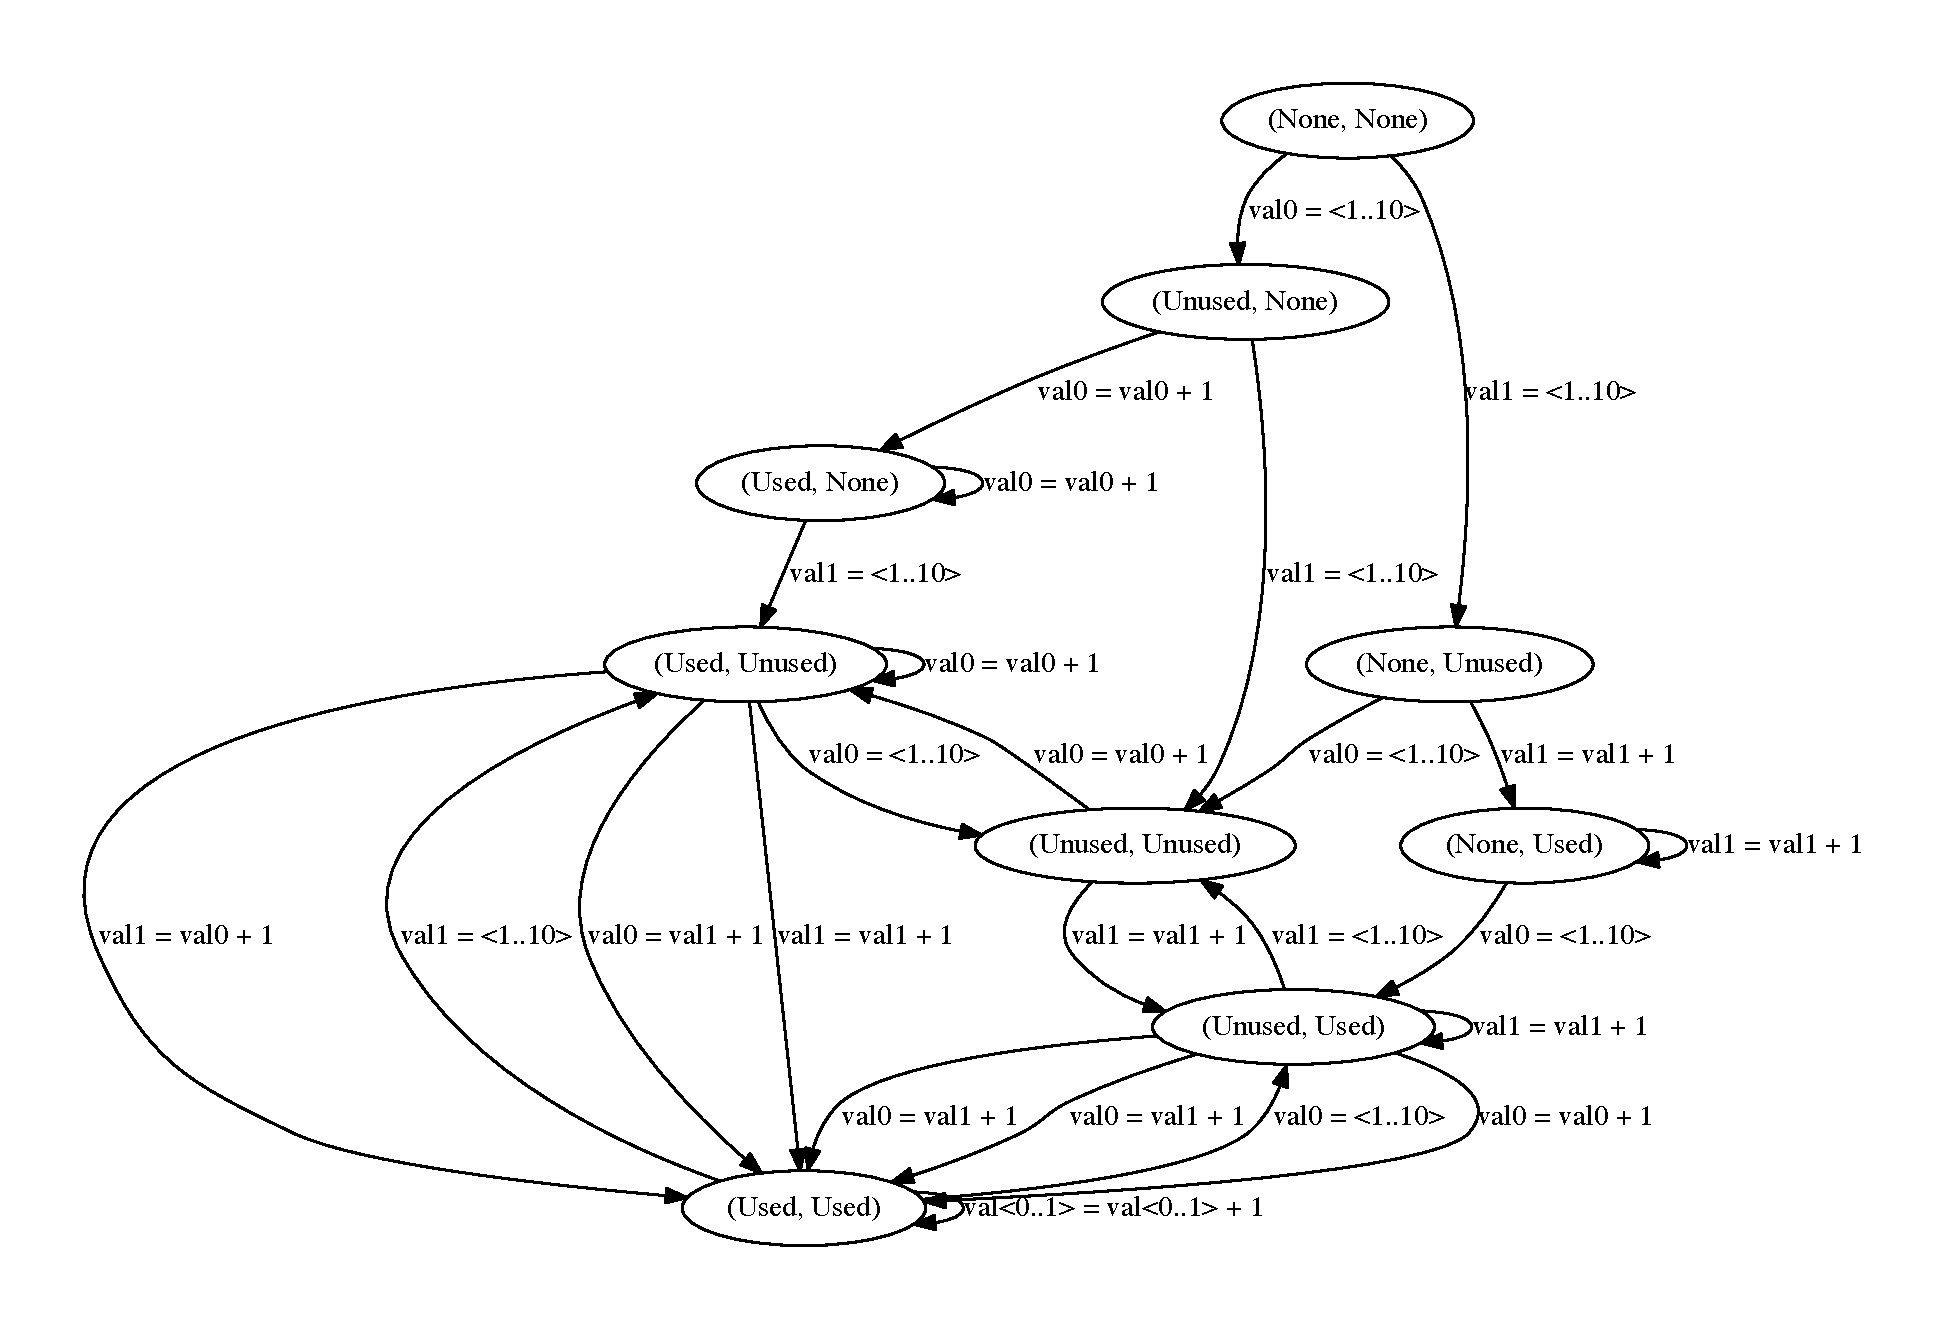
\includegraphics[width=\columnwidth]{states}
\caption{Constraints on actions in a test, based on pool states}
\label{fig:poolacts}
\end{figure}